% Compile with: pdflatex report.tex
\documentclass[12pt,a4paper]{article}
\usepackage[margin=1in]{geometry}
\usepackage{listings}
\usepackage{graphicx}
\usepackage{amsmath}
\usepackage{tabularx}
\usepackage{longtable}
\usepackage[hidelinks]{hyperref}
\usepackage{tikz}
\usetikzlibrary{arrows.meta,automata,positioning}

\title{\textbf{A Report on\\Compiler Design Lab (CS304): Mini Project\\Phase 1}}
\author{
Abhiram Suresh (Roll No: 231CS202)\\
Advaith Nair (Roll No: 231CS205)\\
Arjun Rijesh (Roll No: 231CS212)\\[0.5cm]
\includegraphics[width=6cm]{nitk_logo.png} \\[0.5cm]
\textbf{Department of Computer Science and Engineering}\\
\textbf{National Institute of Technology Karnataka}\\
Surathkal, Mangaluru - 575025\\[0.5cm]
\textbf{15-August-2025}\\[5cm]
}
\date{}

\lstset{
  basicstyle=\ttfamily\small,
  breaklines=true,
  tabsize=2,
  frame=single,
  showstringspaces=false
}

\begin{document}
\maketitle

\section{Introduction}

\subsection{Lexical Analysis}
Lexical analysis is the first phase of the compiler where the source program is scanned from left to right, character by character, and divided into meaningful sequences called \textit{lexemes}. The lexical analyzer produces tokens as output, which are then used by the syntax analyzer.

In our mini-project, we have implemented a lexical analyzer for the C language using \textbf{Flex}. The scanner can recognize:
\begin{itemize}
    \item Identifiers
    \item Preprocessor directives
    \item Keywords
    \item Constants (numeric, string, character)
    \item Operators
    \item Punctuation
    \item Comments (single-line and nested multi-line)
\end{itemize}
It also maintains a rudimentary symbol table and constant table.

\subsection{Tokens \& Lexemes}
\begin{itemize}
    \item \textbf{Token:} A pair consisting of a token name and an optional attribute value that uniquely identifies a sequence of characters.
    \item \textbf{Lexeme:} The actual sequence of characters in the source program that matches the pattern for a token.
\end{itemize}
For example, in:
\begin{lstlisting}[language=C]
int x = 10;
\end{lstlisting}
``int'' is a keyword token, ``x'' is an identifier token, and ``10'' is a constant token.\\[5cm]

\section{DFA Diagram}

\subsection*{Identifier DFA}
\noindent\textbf{Pattern recognized:} \texttt{[A-Za-z\_][A-Za-z0-9\_]*}

\begin{figure}[h]
\centering
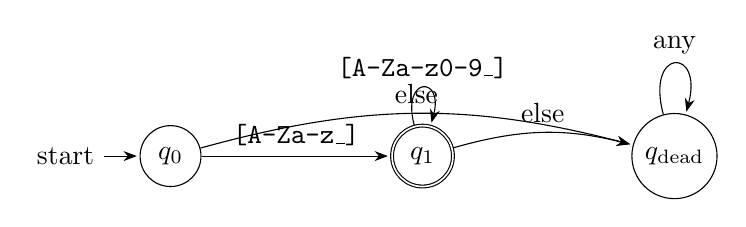
\begin{tikzpicture}[>=Stealth,shorten >=1pt,node distance=3.2cm,on grid,auto]
  \tikzstyle{every state}=[minimum size=22pt]
  % States
  \node[state,initial] (q0) {$q_0$};
  \node[state,accepting,right=of q0] (q1) {$q_1$};
  \node[state,right=of q1] (qd) {$q_{\text{dead}}$};

  % Transitions
  \path[->]
    (q0) edge[above] node{\texttt{[A-Za-z\_]}} (q1)
    (q0) edge[bend left=15,above] node{else} (qd)
    (q1) edge[loop above] node{\texttt{[A-Za-z0-9\_]}} ()
    (q1) edge[bend left=15,above] node{else} (qd)
    (qd) edge[loop above] node{any} ();
\end{tikzpicture}
\caption{DFA for recognizing identifiers}
\end{figure}

\subsubsection*{Explanation}
\begin{itemize}
  \item $q_0$ (start, non-accepting): On a letter or underscore, move to $q_1$; otherwise go to dead.
  \item $q_1$ (accepting): Consume letters, digits, or underscores staying in $q_1$. On any other character, transition to dead (in practice, the scanner \emph{stops} the lexeme before that character and leaves it to the next token).
  \item $q_{\text{dead}}$: Sink state for non-matching strings.
\end{itemize}

\subsubsection*{Notes}
\begin{itemize}
  \item This DFA intentionally treats keywords as \emph{post-processing}: first match as an identifier, then check the lexeme against the keyword table to reclassify.
  \item This matches your scanner rule: \texttt{[A-Za-z\_][A-Za-z0-9\_]*}. (Unicode identifiers and universal character names are out of scope here.)
\end{itemize}

% (Optional) Transition table, if you want it too:
\begin{table}[h]
\centering
\begin{tabular}{c|c|c|c}
\textbf{State} & \textbf{[A-Za-z\_]} & \textbf{[0-9]} & \textbf{else} \\
\hline
$q_0$ & $q_1$ & $q_{\text{dead}}$ & $q_{\text{dead}}$ \\
$q_1$ & $q_1$ & $q_1$ & $q_{\text{dead}}$ \\
$q_{\text{dead}}$ & $q_{\text{dead}}$ & $q_{\text{dead}}$ & $q_{\text{dead}}$ \\
\end{tabular}
\caption{Transition table for the Identifier DFA}\\[5cm]
\end{table}

\section{Results}

\subsection*{Test Case 1}
\textbf{Input:}
\begin{lstlisting}[language=C]
int main() {
    const int x = 10;
    const float y = 3.1415;
    return x + y;
}
\end{lstlisting}

\textbf{Output:}
\begin{itemize}
    \item Keywords: \texttt{int}, \texttt{const}, \texttt{return}
    \item Identifiers: \texttt{main}, \texttt{x}, \texttt{y}
    \item Constants: \texttt{10}, \texttt{3.1415}
\end{itemize}

\textbf{Symbol Table:}
\begin{tabularx}{\linewidth}{|l|l|l|l|}
\hline
\textbf{Name} & \textbf{Type} & \textbf{Line Number} & \textbf{Qualifier} \\
\hline
main & function & 1 & - \\
x & int & 2 & const \\
y & float & 3 & const \\
10 & int & 2 & - \\
3.1415 & float & 3 & - \\
\hline
\end{tabularx}

\subsection*{Test Case 2}
\textbf{Input:}
\begin{lstlisting}[language=C]
#include <stdio.h>

int sum(int a, int b) {
    return a + b;
}

int main() {
    int result = sum(5, 7);
    printf("Sum is %d\n", result);
    return 0;
}
\end{lstlisting}

\textbf{Output:}
\begin{itemize}
    \item Preprocessor: \texttt{\#include <stdio.h>}
    \item Keywords: \texttt{int}, \texttt{return}
    \item Identifiers: \texttt{sum}, \texttt{a}, \texttt{b}, \texttt{main}, \texttt{result}, \texttt{printf}
    \item Constants: \texttt{5}, \texttt{7}, \texttt{"Sum is \%d\textbackslash n"}
\end{itemize}


\textbf{Symbol Table:}
\begin{tabularx}{\linewidth}{|l|l|l|l|}
\hline
\textbf{Name} & \textbf{Type} & \textbf{Line Number} & \textbf{Qualifier} \\
\hline
sum & function & 3 & - \\
a & int & 3 & parameter \\
b & int & 3 & parameter \\
main & function & 7 & - \\
result & int & 8 & - \\
5 & int & 8 & - \\
7 & int & 8 & - \\
"Sum is \%d\textbackslash n" & string & 9 & - \\
\hline
\end{tabularx}
\section*{Appendix}
\subsection*{Flex Source (\texttt{scanner.l})}
\lstinputlisting[language=C]{../src/scanner.l}

\subsection*{Build Script}
\lstinputlisting[language=make]{../src/Makefile}

\subsection*{Sample Inputs}
\lstinputlisting[language=C]{../tests/simple.c}
\lstinputlisting[language=C]{../tests/functions.c}

\end{document}
